\documentclass{uinsaintekskripsi}

%-----------------------------------------------------------------
%Disini awal masukan untuk data Skripsi (ISI SESUAI DENGAN DATA ANDA!)
%-----------------------------------------------------------------
\titleind{
JUDUL SKRIPSI JUDUL SKRIPSI JUDUL SKRIPSI
}

\titleeng{
TITLE TITLE TITLE
}


\fullname{NAMA LENGKAP}
\NIM{00000000}

\studyprogramme{Teknik Informatika}
\yearsubmit{0000}



\begin{document}
\cover\titlepage

\pengesahanscan
\persetujuanscan
\declarepagescan

%-----------------------------------------------------------------
%Disini awal masukan untuk Kata Pengantar (ISI SESUAI DENGAN DATA ANDA!)
%-----------------------------------------------------------------
\preface
Kata Pengantar Kata Pengantar Kata Pengantar Kata Pengantar Kata Pengantar Kata Pengantar Kata Pengantar Kata Pengantar Kata Pengantar Kata Pengantar Kata Pengantar Kata Pengantar Kata Pengantar Kata Pengantar Kata Pengantar Kata Pengantar Kata Pengantar Kata Pengantar Kata Pengantar Kata Pengantar Kata Pengantar.

Kata Pengantar Kata Pengantar Kata Pengantar Kata Pengantar Kata Pengantar Kata Pengantar Kata Pengantar Kata Pengantar Kata Pengantar Kata Pengantar Kata Pengantar Kata Pengantar Kata Pengantar.
\vspace{0.8cm}

\begin{tabular}{p{7cm}l}
&Yogyakarta, 00 Bulan 0000\\
&\\
&\\
&Penulis
\end{tabular}
%-----------------------------------------------------------------
%-----------------------------------------------------------------

%-----------------------------------------------------------------
%Halaman Persembahan (ISI SESUAI DENGAN DATA ANDA!)
%-----------------------------------------------------------------
\acknowledment
\begin{flushright}
\Large\emph\cal{Karya sederhana ini penulis persembahkan \\
untuk ............................. tercinta}
\end{flushright}
%-----------------------------------------------------------------
%-----------------------------------------------------------------


%-----------------------------------------------------------------
%Halaman Motto (ISI SESUAI DENGAN DATA ANDA!)
%-----------------------------------------------------------------
\motto
\emph{"Kami telah turunkan kepadamu Al-Dzikir (Al-Quran)
untuk kamu terangkan kepada manusia apa-apa  yang diturunkan kepada
mereka agar mereka berpikir"}
\begin{flushright}
(QS. 16:44)
\end{flushright}
%-----------------------------------------------------------------
%-----------------------------------------------------------------


%-----------------------------------------------------------------
%Daftar Isi (TIDAK PERLU DIUBAH)
%-----------------------------------------------------------------
\newpage\phantomsection\addcontentsline{toc}{chapter}{DAFTAR ISI}
\makeatletter\renewcommand\l@chapter[2]{\ifnum \c@tocdepth >\z@\addpenalty\@secpenalty\addvspace{0em}\setlength\@tempdima{1.4em}\begingroup\parindent \z@ \rightskip \@pnumwidth\parfillskip -\@pnumwidth\leavevmode \bfseries\advance\leftskip\@tempdima\hskip -\leftskip#1\nobreak\ \leaders\hbox{$\m@th\mkern \@dotsep mu\hbox{.}\mkern \@dotsep mu$}\hfil\nobreak\hb@xt@\@pnumwidth{\hss #2}\par\endgroup\fi}\makeatother
\begin{onehalfspacing}\tableofcontents\end{onehalfspacing}
%-----------------------------------------------------------------
%-----------------------------------------------------------------

%-----------------------------------------------------------------
%Daftar Tabel (JIKA DIPERLUKAN, HAPUS KARAKTER % SEBELUM \newpage dan \begin)
%-----------------------------------------------------------------
\newpage\phantomsection\addcontentsline{toc}{chapter}{DAFTAR TABEL}
\begin{onehalfspacing}\listoftables\end{onehalfspacing}
%-----------------------------------------------------------------
%-----------------------------------------------------------------

%-----------------------------------------------------------------
%Daftar Gambar (JIKA DIPERLUKAN, HAPUS KARAKTER % SEBELUM \newpage dan \begin)
%-----------------------------------------------------------------
\newpage\phantomsection\addcontentsline{toc}{chapter}{DAFTAR TABEL}
\begin{onehalfspacing}\listoffigures\end{onehalfspacing}
%-----------------------------------------------------------------
%-----------------------------------------------------------------


%-----------------------------------------------------------------
%Daftar Lambang (ISI SESUAI DENGAN DATA ANDA!)
%-----------------------------------------------------------------
\lambang
\begin{tabular}{cp{10.5cm}}
  $x\in A$ & : $x$ anggota A\\
  $A\subseteq X$ & : A himpunan bagian (\textit{subset}) atau sama dengan X\\
  $\mathbb{N}$ & : himpunan semua asli\\
  $\mathbb{Z}$ & : himpunan semua bilangan bulat\\
  $\mathbb{Z}^{+}$ & : himpunan semua bilangan bulat positif\\
  $\mathbb{R}$ & :himpunan semua bilangan real\\
  $C^{n}_{r}$ & : $r-$kombinasi dari $n$ unsur yang berbeda\\
  $\blacksquare$ & : akhir suatu bukti\\
  $\qed$\hfill & : akhir suatu contoh\\
  $\rightarrow$ & : menuju\\
  $\displaystyle\sum_{i=1}^{n}{a_{i}}$ & : penjumlahan $a_{1}+a_{2}+\cdots + a_{n}$\\
  $\displaystyle\prod_{i=1}^{n}{a_{i}}$ & : perkalian $a_{1}\cdot a_{2}\cdot\cdots \cdot a_{n}$\\
  $p \Rightarrow q$ & : jika $p$ maka $q$\\
  $\Leftrightarrow$ & : jika dan hanya jika\\
  $x\leftarrow a$ & : nilai $a$ dimasukkan ke $x$
\end{tabular}
%-----------------------------------------------------------------
%-----------------------------------------------------------------


%-----------------------------------------------------------------
%Disini awal masukan Intisari (ISI SESUAI DENGAN DATA ANDA!)
%-----------------------------------------------------------------
\begin{abstractind}
Intisari Intisari Intisari Intisari Intisari Intisari Intisari Intisari Intisari Intisari Intisari Intisari Intisari Intisari Intisari Intisari Intisari Intisari Intisari Intisari Intisari Intisari Intisari Intisari Intisari Intisari Intisari Intisari Intisari Intisari Intisari Intisari Intisari Intisari Intisari Intisari Intisari Intisari Intisari Intisari Intisari Intisari Intisari Intisari Intisari Intisari Intisari Intisari Intisari Intisari Intisari Intisari Intisari Intisari Intisari Intisari Intisari Intisari Intisari.
\end{abstractind}
%-----------------------------------------------------------------
%-----------------------------------------------------------------

%-----------------------------------------------------------------
%Disini awal masukan untuk Abstract (ISI SESUAI DENGAN DATA ANDA!)
%-----------------------------------------------------------------
\begin{abstracteng}
Abstract Abstract Abstract Abstract Abstract Abstract Abstract Abstract Abstract Abstract Abstract Abstract Abstract Abstract Abstract Abstract Abstract Abstract Abstract Abstract Abstract Abstract Abstract Abstract Abstract Abstract Abstract Abstract Abstract Abstract Abstract Abstract Abstract Abstract Abstract Abstract Abstract Abstract Abstract Abstract Abstract Abstract Abstract Abstract Abstract Abstract Abstract Abstract Abstract Abstract Abstract Abstract Abstract Abstract Abstract Abstract Abstract Abstract Abstract.
\end{abstracteng}
%-----------------------------------------------------------------
%-----------------------------------------------------------------

%-----------------------------------------------------------------
%Disini awal masukan untuk Bab (ISI BAB I DAPAT DIEDIT DI FILE Bab1.tex,
%ISI BAB II DAPAT DIEDIT DI FILE Bab2.tex, dst...)
%-----------------------------------------------------------------
\chapter{PENDULUAN}
\section{Latar Belakang}
Teks teks teks teks teks teks teks teks teks teks teks teks teks teks teks teks teks teks teks teks teks teks teks teks teks teks teks teks teks teks teks teks teks teks teks teks teks teks teks teks... dsadas dsads adsad asdsa d sad as dsa dsad s das dsadsad sadas 


\begin{contoh}
Teks teks teks teks teks teks teks teks teks teks teks teks teks teks teks teks teks teks teks teks teks teks teks teks teks tek
\end{contoh}

\begin{contoh}
Teks teks teks teks teks teks teks teks teks teks teks teks teks teks teks teks teks teks teks teks teks teks teks teks teks tek
\end{contoh}

\begin{teorema}
Teks teks teks teks teks teks teks teks teks teks teks teks teks teks teks teks teks teks teks teks teks teks teks teks teks tek
\end{teorema}

Teks teks teks teks teks teks teks teks teks teks teks teks teks teks teks teks teks teks teks teks teks teks teks teks teks teks teks teks teks teks teks...

\section{coba}
Teks teks teks teks teks teks teks teks teks teks teks teks teks teks teks teks teks teks teks teks teks teks teks teks teks teks teks teks teks teks teks teks teks teks teks teks teks teks teks teks... dsadas dsads adsad asdsa d sad as dsa dsad s das dsadsad sadas 


\section{Rumusan Masalah}


\section{Batasan Masalah}

\section{Tujuan Penelitian}

\section{Manfaat Penelitian}


\section{Sistematika Penulisan}

\chapter{JUDUL BAB}

\chapter{JUDUL BAB...}
Contoh gambar..
\begin{figure}[H]
\centering
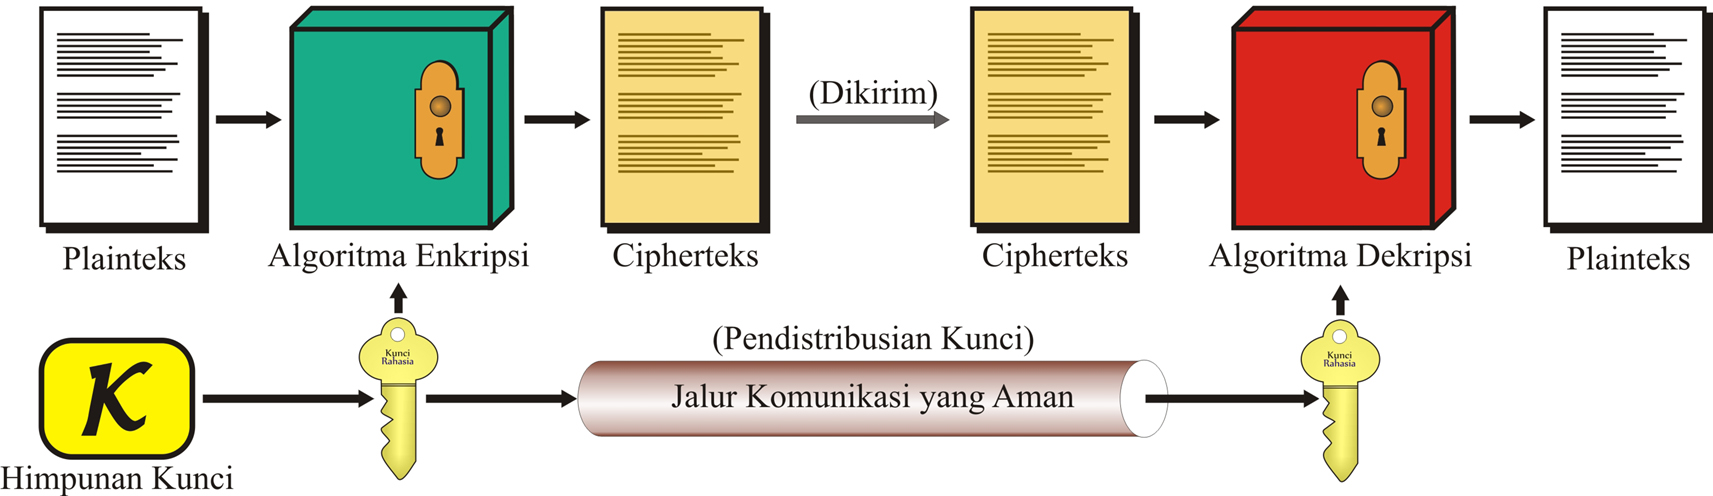
\includegraphics[width=12cm]{skemasimetris}
\caption{Diagram ilustrasi}
\end{figure}
\bigskip
\begin{figure}[H]
\centering
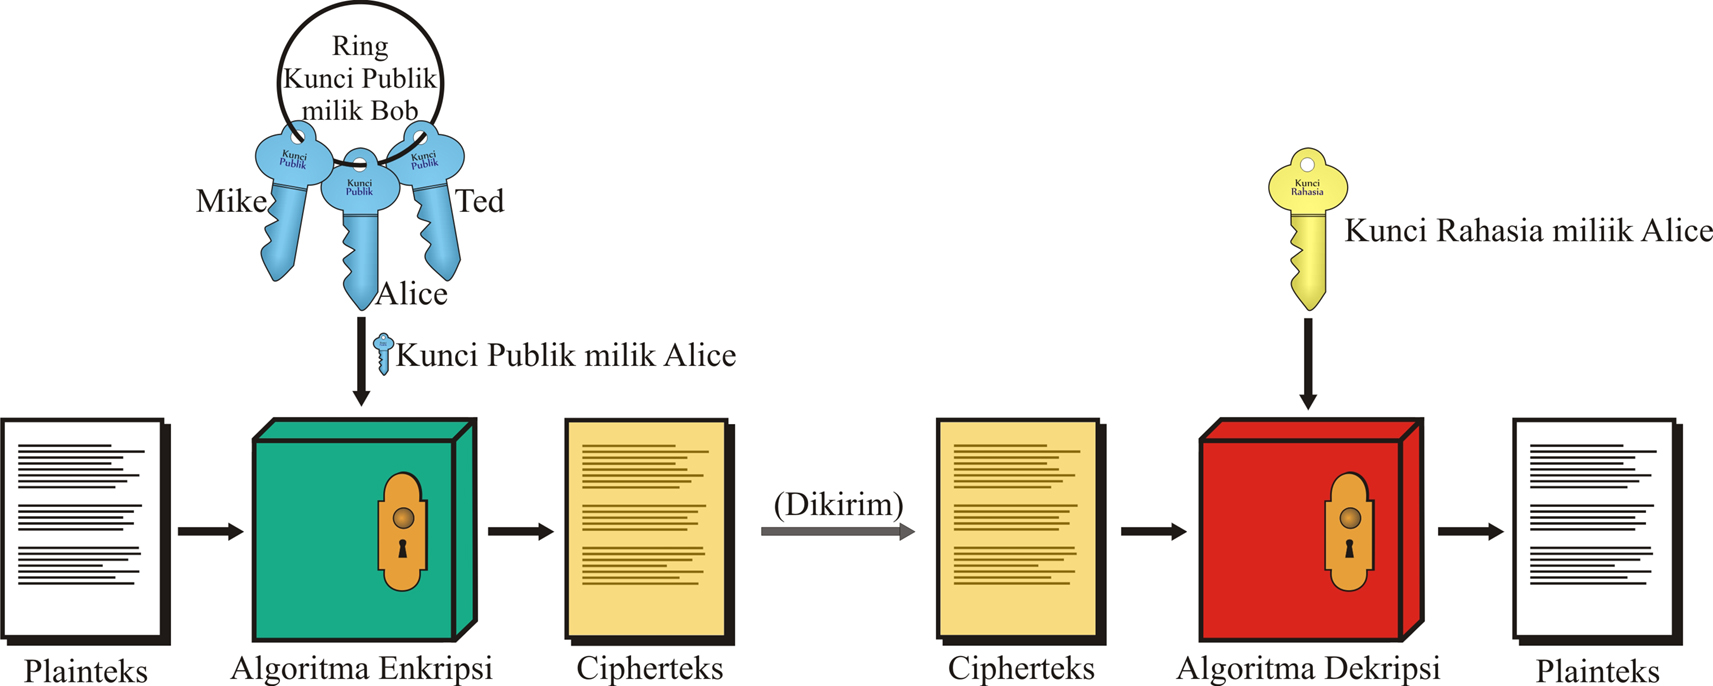
\includegraphics[width=12cm]{skemaasimetris}
\caption{Diagram ilustrasi}
\end{figure}

Contoh tabel...
\begin{longtable}{|c|c|c|c|c|}
 \caption{Hasil Panen Padi}\label{tran7}\\
 \hline
  Kota Jogja&Bantul&Sleman&Kulon Progo&Gunung Kidul \\
  \hline
  55 & 164 & 91 & 239 & 921 \\
  \hline
  13 & 70 & 187 & 295 & 629 \\
  \hline
  3 & 96 & 37 & 525 & 645 \\
  \hline
  6 & 221 & 61 & 175 & 666 \\
  \hline
  64 & 84 & 4 & 133 & 571 \\
  \hline
  50 & 5 & 20 & 259 & 257 \\
  \hline
  33 & 3 & 396 & 749 & 461 \\
  \hline
  10 & 6 & 41 & 43 & 535 \\
  \hline
  33 & 22 & 108 & 370 & 840 \\
  \hline
  & 77& 398 & 321 & 857 \\
  \hline
  & 250 & 172 & 474 & 402 \\
  \hline
  & 167 & 111 & 327 & 57 \\
  \hline
  & 17 & 328 & 225 & 299 \\
  \hline
  & 30 & 7 & 346 & 644 \\
  \hline
  &  & 28 & 455 & 1.984 \\
  \hline
  &  & 224 & 143 &  \\
  \hline
  &  & 63 & 256 &  \\
  \hline
  &  & 146 & 190 &  \\
  \hline
  &  & 69 & 436 &  \\
  \hline
  &  & 254 & 62 &  \\
  \hline
  &  & 192 & 528 &  \\
  \hline
\end{longtable}


\begin{longtable}{|ccccccc|}
\caption{Penduduk dan Pertumbuhannya }\label{tran3}\\
\hline
 \multicolumn{3}{|c}{Penduduk Bantul} & & \multicolumn{3}{c|}{Penduduk Sleman} \\
  \hline
   Tahun  &   Penduduk    &   Pertumbuhan   &    &  Tahun    &  Penduduk     & Pertumbuhan\\
  \hline
  1990 & 1,86  &      &    & 1990 & 22,16  &  \\
  1992 & 2,34  & 0,48 &    & 1992 & 29,13  & 6,97 \\
  1994 & 2,78  & 0,44 &    & 1994 & 37,21  & 8,08\\
  1996 & 3,21  & 0,43 &    & 1996 & 48,28  & 11,07 \\
  1998 & 4,22  & 1,01 &    & 1998 & 60,12  & 11,84\\
  2000 & 6,21  & 1,99 &    & 2000 & 74,51  & 14,39\\\hline
\end{longtable}
\chapter{JUDUL BAB...}

\chapter{JUDUL BAB}
%-----------------------------------------------------------------
%Disini akhir masukan Bab
%-----------------------------------------------------------------

%-----------------------------------------------------------------
%Disini awal masukan untuk Daftar Pustaka (ISI SESUAI DENGAN DATA ANDA!)
%-----------------------------------------------------------------
\begin{thebibliography}{99}
\addcontentsline{toc}{chapter}{DAFTAR PUSTAKA}
\bibitem[Anderson(1951)]{anderson}
Anderson,  T.F., 1951, Techniques  for  the  Preservation  of  Three
Dimensional  Structure  in  Preparing  Specimens  for  the  Electron
Microscope. Trans. N. YAcad. Sci. 13:130-134.

\bibitem[Andrew (1961)]{andrew}
Andrew, Jr., 1961. Studies in Paleobotany. John Wiley \& Sons, Inc., New
York.
\end{thebibliography}
%-----------------------------------------------------------------
%-----------------------------------------------------------------


%-----------------------------------------------------------------
%Disini awal masukan untuk Lampiran (JIKA DIPERLUKAN)
%-----------------------------------------------------------------
\appendix
\chapter{SKRIP PROGRAM JAVA}
\lstset{language=java, frame=single}
\lstset{numbers=left, numberstyle=\tiny, stepnumber=1, numbersep=5pt, basicstyle=\footnotesize}
\lstset{frame=shadowbox, xleftmargin=6pt, xrightmargin=8pt, rulesepcolor=\color{black}}
\lstset{keywordstyle=\color{blue},breaklines=true, breakindent=27pt}
\lstinputlisting{Main.java}


\chapter{TABEL KODE ASCII}
\begin{figure}[H]
\centering
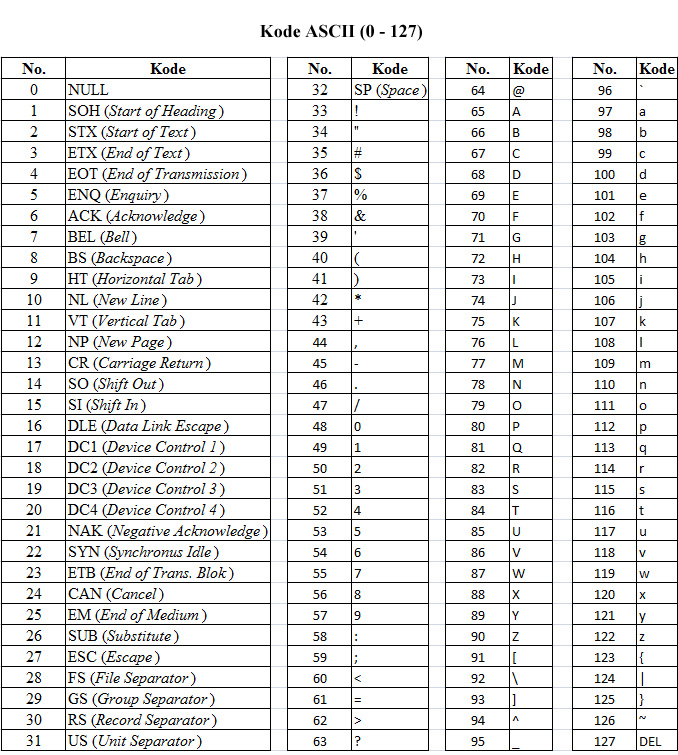
\includegraphics[width=14cm]{ASCIIreguler}
\end{figure}
%-----------------------------------------------------------------
%-----------------------------------------------------------------
\end{document}
